 \section{\tc Architecture and Security Model}

%In this section, we discuss the general design of \tc. First we present a strawman system design that illustrates some of the technical challenges that arise in the design of \tc. We then present our \tc architecture, describing the front-end (blockchain) and back-end (off-chain) components, and give a high-level view of the security model underpinning our design.

\iffalse{
\subsection{Strawman design}

Here we sketch a simple (but, as we show, na\"{i}ve) strawman design that provides authenticated data feeds along with accompanying attestations. 

%To harmonize with terminology introduced shortly in the paper, we refer to the untrusted component of a \tc host as the \medname and the code running in an SGX enclave as the \encname.

The strawman solution is as follows:

\begin{itemize}[leftmargin=5mm]
\item
{\bf Monitor and relay.}
The \tc system
monitors the blockchain for 
datagram requests. A contract \reqcont 
requests a datagram by including a distinguished message in its state (e.g., ``\tc service \#123 request:''), along with
a specification \dgform of the requested datagram.
Monitoring happens in the untrusted part of the \tc server, which controls the network stack. Any scraped specification \dgform is passed to a (trusted) enclave process.
\item
{\bf Securely fetch feed.}
Based on the \dgform, the trusted enclave process contacts a data source, establishing an HTTPS channel to a suitable target web page $\weburl$ (which might, e.g., be specified in \dgform). 
The process verifies that the validity of the certificate for the host serving \weburl.
It then fetches page contents, parses them, and extracts a datagram \dgm as specified in \dgform.

Finally, the enclave process produces an attestation $\att$ on: its code in the enclave, $\dgform$, a timestamp $T$ on the fetched data, and $\dgm$. 
It sends $\att$ to $\reqcont$.
\item
{\bf Verify}.
\reqcont verifies the attestation $\att$. If successful, \reqcont consumes \dgm (potentially matching \dgform against an internal queue of datagram requests).
\end{itemize}

This strawman scheme has a few nice features: conceptual simplicity, no need to maintain a \tc contract on the blockchain, and the ability for \reqcont to check the freshness of \att. It has a few serious drawbacks, however.

\paragraph{Problems with the strawman scheme.}
Our strawman scheme is unworkable for several reasons. First, verification of \att in the requesting contract \reqcont is not practical. Although SGX provides a 
trusted clock, the clock does not provide absolute time, but only time relative to a host-specific reference point.
Thus it is not clear in our strawman scheme how to produce a timestamp $T$ in absolute time. Furthermore, in Ethereum, opcodes for in-contract cryptographic operations are very limited and do not support the proprietary EPID group-signature scheme present in SGX attestations. While achievable in principle, as the Ethereum virtual machine is Turing-complete, verification of attestations would impose prohibitively expensive gas costs on \reqcont. 

To address these problems, our \tc architecture supports only off-chain verification of attestations.

Another problem with our strawman scheme is that it lacks an on-blockchain mechanism to enforce payment for datagrams. It is desirable for \tc to accept payments via a smart contract in order to permit payment in the system's cryptocurrency (e.g., Ether) and to ensure a {\em fair exchange} between payments and datagrams. Even a not-for-profit \tc service might accept small gas payments to cover the cost of datagram transmission. Without enforcement of fair exchange, relying contracts or the \tc service would risk being defrauded by the other party. \tc could attempt to deliver datagrams only to contracts whose code guarantees payment to \tc, but verifying this property even in templated code would be challenging, given the many complicated dependencies in a smart-contract system (e.g., a contract might attempt to make payment but lack gas or ether). 

To address these problems, our \tc architecture uses a smart contract \tcont as a blockchain front end.
\fi

The \tcs system includes three main components: The \tcontract (\tcont), the \encname (\engine), and the \medname (\relay). The \encname and \medname reside on the \tc server, while the \tcontract  resides on the blockchain. An architectural schematic showing the roles of these components is given in Figure~\ref{fig:overview}.

\vspace{-2mm}
\begin{figure}[h!]
\centering
\begin{tikzpicture}
  [entity/.style={rectangle,draw=black,minimum height=3.5em,text width=3.5em,align=center},
   contract/.style={entity,text width=5.7em},
   trusted/.style={fill=green!30},
   communication/.style={blue,ultra thick,text=black},
   bg-box/.style={rectangle,rounded corners,draw=black,dashed}]
  \node[contract,trusted] (ctc) {TC Contract\\$\tcont$};
  \node[contract,fill=white,below=1.5em of ctc] (cu) {User Contract\\$\reqcont$};
  \node[entity,fill=none,right=2.5em of ctc] (relay) {Relay};
  \node[entity,trusted,right=2.5em of cu] (enc) {Enclave};

  \begin{pgfonlayer}{background}
    \node[bg-box,
          fill=yellow!20,
          fit={($(ctc.north east)+(0.25em,0.25em)$)($(cu.south west)+(-0.25em,-0.25em)$)},
          label=above:{\bf Blockchain}] (blockchain) {};
    \node[bg-box,
          fill=black!20,
          fit={($(relay.north east)+(0.25em,0.25em)$)($(enc.south west)+(-0.25em,-0.25em)$)},
          label=above:{\bf TC Server}] (tc) {};
  \end{pgfonlayer}

  \node[right=-0.15em of tc,color=red,transform canvas={yshift=2.5em}] (https) {\scriptsize \bf HTTPS};
  \node[rectangle,draw=black,fill=red!20,right=2.75em of tc,minimum height=9.75em,label=above:{\bf Data Source}] (data) {\scriptsize \tt LotsOData.com};

  \draw[stealth-stealth,communication] ([xshift=-0.75em,yshift=-0.75em]ctc.east) -| ([xshift=-0.75em,yshift=-0.75em]enc.north);
  \draw[stealth-stealth,communication] ([yshift=0.75em]ctc.south) -- ([yshift=-0.75em]cu.north);
  \draw[stealth-stealth,communication] ([xshift=0.75em,yshift=-0.75em]enc.north) |- ([xshift=0.75em,yshift=1.75em]data.west);
\end{tikzpicture}
\caption{{\bf Basic Town Crier architecture.}}
\label{fig:overview}
\end{figure}

%\begin{figure}[h!]
%\centering
%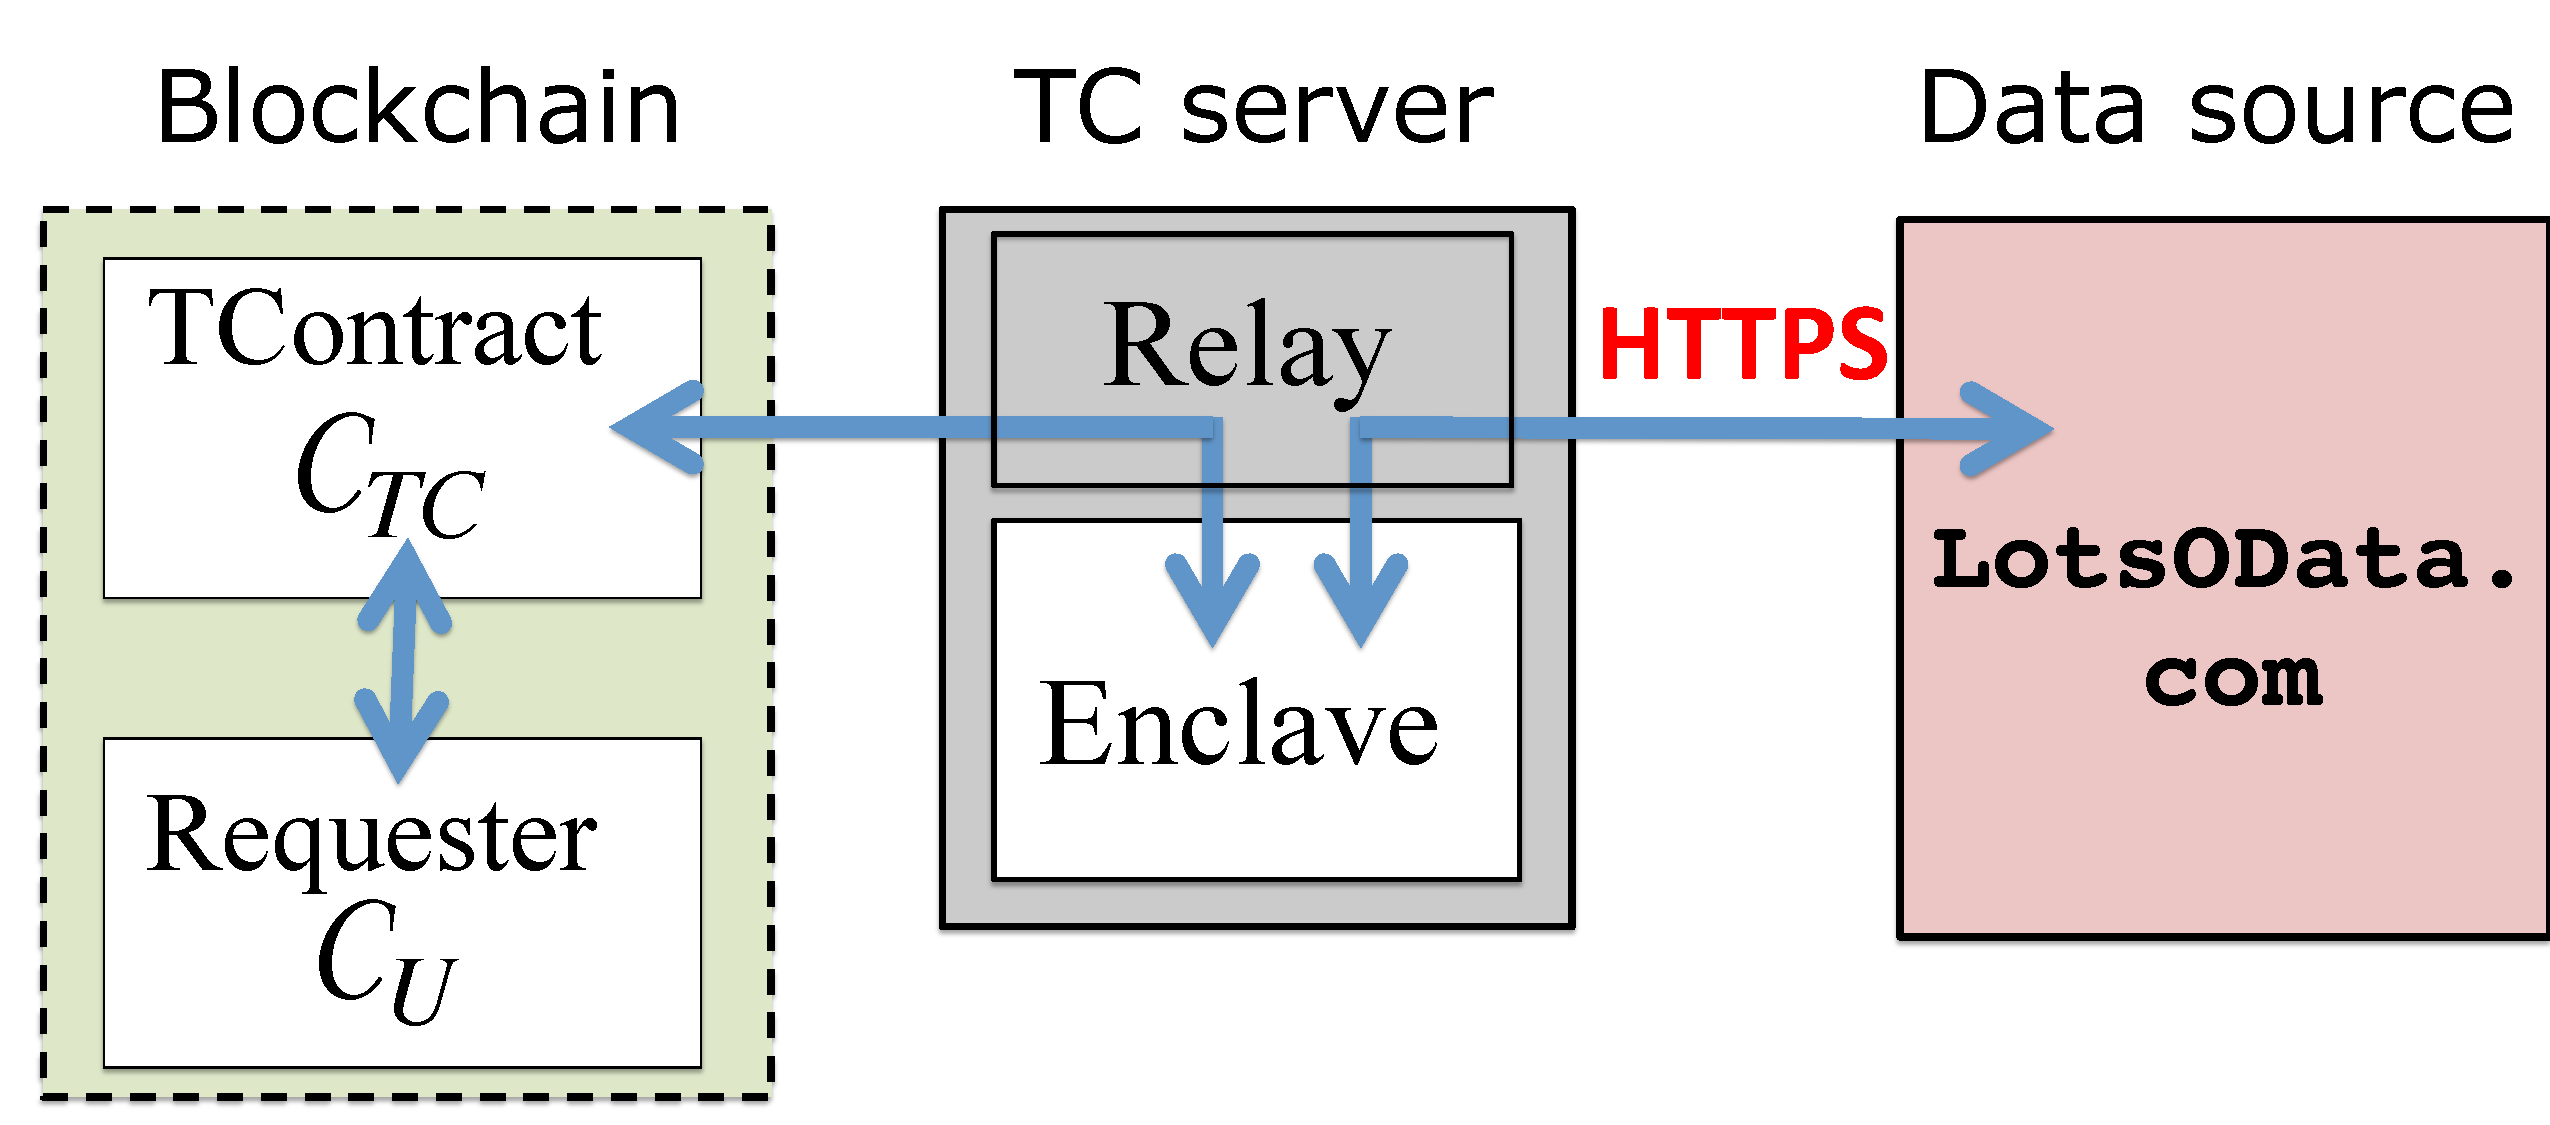
\includegraphics[width=\columnwidth]{figures/OverviewFig}
%\caption{{\bf Basic Town Crier architecture.}}
%\label{fig:overview}
%\end{figure}
\vspace{-2mm}

\paragraph{The \tcontract \tcont.} The \tcontract (denoted by \tcont) is a smart contract that acts as the blockchain front end of the \tc service. It is designed to present a simple API to a relying contract \reqcont for its requests from \tc. Very simply, \tcont accepts datagram requests from a requester \reqcont and returns corresponding datagrams from \tc. Additionally, \tcont manages \tc monetary resources, which in Ethereum take the form of ether (money) and gas (``fuel'' for contracts).

\paragraph{The \encname \engine.}
We refer to the TC code running in the SGX enclave simply as the \encname. In TC, the \encname ingests and fulfills datagram requests from the blockchain. To obtain the data for inclusion in datagrams, it queries external data sources, specifically HTTPS-enabled internet services. It returns a datagram to a requesting contract \reqcont as a digitally signed blockchain message. Under our assumed security model for SGX, apart from its network functions, the \encname runs in complete isolation from an adversarial OS as well as other process on the host. 

\paragraph{The \medname \relay.} As an SGX enclave process, the \encname lacks direct network access. Thus the \medname handles bidirectional network traffic on behalf of the \encname. Specifically, the \medname provides network connectivity from the \encname to three different types of entities: 

\begin{enumerate}
\item {\em The Blockchain (the Ethereum system):}  The \medname scrapes the blockchain in order to monitor the state of the \tcontract  \tcont. In this way, it performs implicit message passing from \tcont to the \encname, as neither component itself has network connectivity. Additionally, the \medname places messages emitted from the \encname (datagrams) on the blockchain.
\item {\em Clients:} The \medname runs a web server to handle off-chain service requests from clients, specifically, requests for attestations from the \encname. As we soon explain, an attestation provides a unique public key for the \encname instance to the  client and proves that the \encname is executing correct code in an enclave and that its clock is correct in terms of absolute (wall-clock time). A client that successfully verifies an attestation can then safely create a relying contract \reqcont that uses the \tc.
\item {\em Data sources:} The \medname relays traffic to and from data sources (HTTPS-enabled servers) queried by the \encname. 
\end{enumerate}

The \medname is an ordinary user-space application. It does not benefit from integrity protection by SGX and thus, unlike the \encname, can be subverted by an adversarial OS on the \tc server, causing network delays or failures. A key design aim of \tc, however, is that \medname should be unable to cause incorrect datagrams to be produced or users to lose fees paid to \tc for datagrams (although they may lose gas used to fuel their requests). As we shall show, in general the \medname~{\em can only mount denial-of-service attacks against \tc}. 

\paragraph{Security model}

Here we give a brief overview of our security model for \tc, providing more details in later sections. We assume the following:

\begin{itemize}

\item {\em Blockchain communication.} Transaction and message sources are authenticable, i.e., a transaction $m$ sent from an account ${\cal P}_{X}$ (or message $m$ from contract ${\cal C}_{X}$) is identified by the receiving account as originating from $X$. Transactions and messages are integrity protected (as they are digitally signed by the sender), but not confidential. 

\item {\em \encname security:} We make three assumptions about \encname : (1) The \encname behaves honestly, i.e., correctly executes the \tc protocol; (2) The private key $\skTC$ is known only to the \encname; and (3) The \encname has an accurate (internal) real-time clock. (Specifically, the clock is accurate to within \ari{XXX}, as we show experimentally.)  We explain in the next section how we achieve these properties through use of SGX and how the public key $\pkTC$ may be bound to an Ethereum account, given the \encname an authenticable blockchain presence. 

\item {\em Network communication.} The \medname (and other untrusted components of the \tc server) can tamper with or delay communications to and from the \encname. (As we explain in our SGX security model, the \medname cannot otherwise observe or alter the behavior of the \encname.) Thus the \medname is subsumed by an adversary that controls the network. 

\end{itemize}












